{\setbeamertemplate{background}{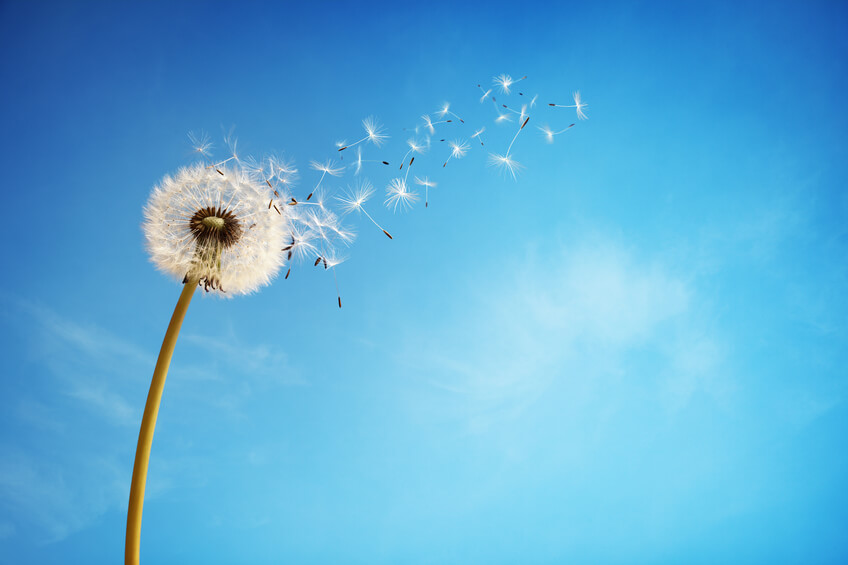
\includegraphics[width=\paperwidth]{fig/leon}}
\begin{frame}
\Huge
\centering \textbf{Demostraci�n.}
\end{frame}}
%%%%%%%%%%%%%%%%%%%%%%%%%%%%%%%%%%%%%%%%%%%%%%%%%%%%%%%55\section{Estrategia}
\section{Demostraci�n }
\begin{frame}

\frametitle{Demostraci�n }
\begin{figure}[!ht]
\begin{flushleft}
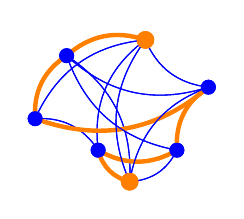
\begin{tikzpicture}[scale=0.1]

\draw[-,color=blue] (14,2) to [bend left] (10,6);
\draw[-,color=blue] (14,2) to [bend right] (20,6);
\draw[-,color=blue] (10,6) to [bend right] (2,10);
\draw[-, color=blue] (2,10) to [bend left] (6,18);
\draw[-, color=blue] (20,6) to [bend left] (24,14);
\draw[-, color=blue] (6,18) to [bend left] (16,20);
\draw[-,color=blue] (16,20) to [bend right] (24,14);

\draw[-,color=blue] (16,20) to [bend right] (2,10);
\draw[-,color=blue] (16,20) to [bend right] (10,6);
\draw[-,color=blue] (6,18) to [bend left] (14,2);
\draw[-, color=blue] (2,10) to [bend right] (24,14);
\draw[-, color=blue] (10,6) to [bend right] (20,6);
\draw[-,color=blue] (24,14) to [bend right] (14,2);
\draw[-,color=blue] (16,20) to [bend right] (14,2);
\draw[-,color=blue] (6,18) to [bend right] (20,6);
\draw[-,color=blue] (6,18) to [bend right] (24,14);
\draw[-, color=blue] (10,6) to [bend right] (14,2);

\filldraw[color=orange] (14,2) circle (30pt);
\filldraw[color=blue] (10,6) circle (25pt);
 \filldraw[color=blue] (20,6) circle (25pt);
 \filldraw[color=blue] (2,10) circle (25pt); 
 \filldraw[color=blue] (6,18) circle (25pt);
 \filldraw[color=blue] (24,14) circle (25pt);
\filldraw[color=orange] (16,20) circle (30pt);



\draw[-,color=blue] (14,2) to [bend left] (10,6);
\draw[-,color=blue] (14,2) to [bend right] (20,6);
\draw[-,color=blue] (10,6) to [bend right] (2,10);
\draw[-, >=latex,ultra thick,color=orange] (2,10) to [bend left] (6,18);
\draw[-, >=latex,ultra thick,color=orange] (20,6) to [bend left] (24,14);
\draw[-, >=latex,ultra thick,color=orange] (6,18) to [bend left] (16,20);
\draw[-,color=blue] (16,20) to [bend right] (24,14);

\draw[-,color=blue] (16,20) to [bend right] (2,10);
\draw[-,color=blue] (16,20) to [bend right] (10,6);
\draw[-,color=blue] (6,18) to [bend left] (14,2);
\draw[-, >=latex,ultra thick,color=orange] (2,10) to [bend right] (24,14);
\draw[-, >=latex,ultra thick,color=orange] (10,6) to [bend right] (20,6);
\draw[-,color=blue] (24,14) to [bend right] (14,2);
\draw[-,color=blue] (16,20) to [bend right] (14,2);
\draw[-,color=blue] (6,18) to [bend right] (20,6);
\draw[-,color=blue] (6,18) to [bend right] (24,14);
\draw[-, >=latex,ultra thick,color=orange] (10,6) to [bend right] (14,2);

\filldraw[color=orange] (14,2) circle (30pt);
\filldraw[color=blue] (10,6) circle (25pt);
 \filldraw[color=blue] (20,6) circle (25pt);
 \filldraw[color=blue] (2,10) circle (25pt); 
 \filldraw[color=blue] (6,18) circle (25pt);
 \filldraw[color=blue] (24,14) circle (25pt);
\filldraw[color=orange] (16,20) circle (30pt);

\end{tikzpicture}
%\end{center}
\end{flushleft}
\end{figure}
%\end{flushleft}


Si la gr�fica \textcolor {blue}{$G_m$} tiene una trayectoria hamiltoniana con v�rtice inicial \textcolor {blue}{$v_1$} y v�rtice final \textcolor {blue} {$v_2$}, \pause entonces la gr�fica \textcolor {blue}{$G_n$} tiene un �rbol generador \textcolor {blue}{ $T$} tal que \textcolor {blue} {$d_T(w_i)=d_i$} con \textcolor {blue} {$1\leq i \leq n$}.


\begin{figure}[!ht]
\begin{flushright}


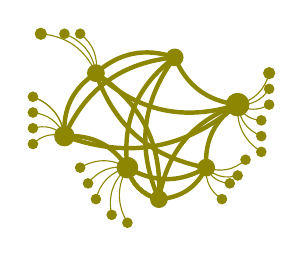
\begin{tikzpicture}[scale=0.1]

\draw[-,>=latex,ultra thick,color=olive] (14,2) to [bend left] (10,6);
\draw[-,>=latex,ultra thick,color=olive] (14,2) to [bend right] (20,6);
\draw[-,>=latex,ultra thick,color=olive] (10,6) to [bend right] (2,10);
\draw[-, >=latex,ultra thick,color=olive] (2,10) to [bend left] (6,18);
\draw[-, >=latex,ultra thick,>=latex,ultra thick,color=olive] (20,6) to [bend left] (24,14);
\draw[-,>=latex,ultra thick, >=latex,ultra thick,color=olive] (6,18) to [bend left] (16,20);
\draw[-,>=latex,ultra thick,color=olive] (16,20) to [bend right] (24,14);

\draw[-,>=latex,ultra thick,color=olive] (16,20) to [bend right] (2,10);
\draw[-,>=latex,ultra thick,color=olive] (16,20) to [bend right] (10,6);
\draw[-,>=latex,ultra thick,color=olive] (6,18) to [bend left] (14,2);
\draw[-, >=latex,ultra thick,color=olive] (2,10) to [bend right] (24,14);
\draw[-, >=latex,ultra thick,color=olive] (10,6) to [bend right] (20,6);
\draw[-,>=latex,ultra thick,color=olive] (24,14) to [bend right] (14,2);
\draw[-,>=latex,ultra thick,color=olive] (16,20) to [bend right] (14,2);
\draw[-,>=latex,ultra thick,color=olive] (6,18) to [bend right] (20,6);
\draw[-,>=latex,ultra thick,color=olive] (6,18) to [bend right] (24,14);
\draw[-, >=latex,ultra thick,color=olive] (10,6) to [bend right] (14,2);





\draw[-,color=olive] (6,18) to [bend right](-1,23);
\draw[-,color=olive] (6,18) to [bend right] (2,23);
\draw[-,color=olive] (6,18) to [bend right] (4,23);




\draw[-,color=olive] (20,6) to [bend right](22,2);
\draw[-,color=olive] (20,6) to [bend right] (23,4);
\draw[-,color=olive] (20,6) to [bend right] (24,5);
\draw[-,color=olive] (20,6) to [bend right] (25,7);


\draw[-,color=olive] (2,10) to [bend right](-2,9);
\draw[-,color=olive] (2,10) to [bend right] (-2,11);
\draw[-,color=olive] (2,10) to [bend right] (-2,13);
\draw[-,color=olive] (2,10) to [bend right] (-2,15);
\draw[-,color=olive] (2,10) to [bend right] (-2,15);




\draw[-,color=olive] (10,6) to [bend right](10,-1);
\draw[-,color=olive] (10,6) to [bend right] (8,0);
\draw[-,color=olive] (10,6) to [bend right] (6,2);
\draw[-,color=olive] (10,6) to [bend right] (5,4);
\draw[-,color=olive] (10,6) to [bend right] (4,6);




\draw[-,color=olive] (24,14) to [bend right](27,8);
\draw[-,color=olive] (24,14) to [bend right] (27,10);
\draw[-,color=olive] (24,14) to [bend right] (27,12);
\draw[-,color=olive] (24,14) to [bend right] (28,14);
\draw[-,color=olive] (24,14) to [bend right] (28,16);
\draw[-,color=olive] (24,14) to [bend right] (28,18);



\filldraw[color=olive] (-1,23) circle (20pt);% node[] {\small \textcolor{black}{$w_3$}};
\filldraw[color=olive] (2,23) circle (17pt);% node[] %{\tiny \textcolor{black}{$w_4$}};
\filldraw[color=olive] (4,23) circle (17pt);% node[] %{\tiny \textcolor{black}{$w_2$}};


\filldraw[color=olive] (-2,9) circle (17pt);% node[] {\tiny \textcolor{black}{$w$}};
\filldraw[color=olive] (-2,11) circle (17pt);% node[] %{\tiny \textcolor{black}{$w_4$}};
\filldraw[color=olive] (-2,13) circle (17pt);% node[] %{\tiny \textcolor{black}{$w_2$}};
\filldraw[color=olive] (-2,15) circle (17pt);% node[] %{\tiny \textcolor{black}{$w_2$}};

\filldraw[color=olive] (10,-1) circle (17pt);% node[] {\tiny \textcolor{black}{$w$}};
\filldraw[color=olive] (8,0) circle (17pt);% node[] %{\tiny \textcolor{black}{$w_4$}};
\filldraw[color=olive] (6,2) circle (17pt);% node[] %{\tiny \textcolor{black}{$w_2$}};
\filldraw[color=olive] (5,4) circle (17pt);% node[] %{\tiny \textcolor{black}{$w_2$}};
\filldraw[color=olive] (4,6) circle (17pt);% node[] %{\tiny \textcolor{black}{$w_2$}};



\filldraw[color=olive] (22,2) circle (17pt);% node[] {\tiny \textcolor{black}{$w$}};
\filldraw[color=olive] (23,4) circle (17pt);% node[] %{\tiny \textcolor{black}{$w_4$}};
\filldraw[color=olive] (24,5) circle (17pt);% node[] %{\tiny \textcolor{black}{$w_2$}};
\filldraw[color=olive] (25,7) circle (17pt);% node[] %{\tiny \textcolor{black}{$w_2$}};


%\filldraw[color=olive] (6,18) circle (30pt) node[] {\tiny \textcolor{black}{$w_{k+1}$}};
%\filldraw[color=olive] (20,6) circle (30pt) node[] {\tiny \textcolor{black}{$w_{k+2}$}};






\filldraw[color=olive] (27,8) circle (17pt);% node[] {\tiny \textcolor{black}{$w$}};
\filldraw[color=olive] (27,10) circle (17pt);% node[] %{\tiny \textcolor{black}{$w_4$}};
\filldraw[color=olive] (27,12) circle (17pt);% node[] %{\tiny \textcolor{black}{$w_2$}};
\filldraw[color=olive] (28,14) circle (17pt);% node[] %{\tiny \textcolor{black}{$w_2$}};
\filldraw[color=olive] (28,16) circle (17pt);% node[] %{\tiny \textcolor{black}{$w_2$}};



\filldraw[color=olive] (16,20) circle (30pt);% node[] {\large \textcolor{black}{$w_1$}};
\filldraw[color=olive] (14,2) circle (30pt);% node[] {\large \textcolor{black}{$w_2$}};
\filldraw[color=olive] (28,18) circle (20pt);% node[] {\small \textcolor{black}{$w_k$}};
\filldraw[color=olive] (6,18) circle (30pt);% node[] {\tiny \textcolor{black}{$w_{k+1}$}};
\filldraw[color=olive] (20,6) circle (30pt);% node[] {\tiny \textcolor{black}{$w_{k+2}$}};
\filldraw[color=olive] (2,10) circle (35pt);% node[] {\tiny \textcolor{black}{$w_{k+i-2}$}};
\filldraw[color=olive] (10,6) circle (37pt);% node[] {\tiny \textcolor{black}{$w_{k+m-3}$}};
\filldraw[color=olive] (24,14) circle (40pt);% node[] {\tiny \textcolor{black}{$w_{k+m-2}$}};
\pause
\filldraw[color=olive] (24,14) circle (40pt);% node[] {\large \textcolor{black}{$w_{n}$}};



\end{tikzpicture}
\end{flushright}
\end{figure}
\end{frame}

%%%%%%%%%%%%%%%%%%%%%%%%%%%%%%%%%%%%%%%%%%%%%%%%%%%%%%%%%%%%%%%%%%%%%%%%%%%%%%%%%%%%%%%%%%%%%%%%%%%%%%%%
%%%%%%%%%%%%%%%%%%%%%%%%%%%%%%%%%%%%%%% F subgrafica a G_n e isomorfa a G_m %%%%%%%%%%%%%%%%%%%%%%%%%%%%%%
\begin{frame}
\frametitle{Demostraci�n. $F$ subgr�fica de $G_n$ y $F\cong G_m$  }

\begin{figure}[!ht]
\begin{flushright}
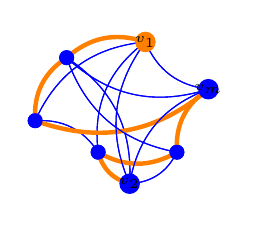
\begin{tikzpicture}[scale=0.1]

\draw[-,color=blue] (14,2) to [bend left] (10,6);
\draw[-,color=blue] (14,2) to [bend right] (20,6);
\draw[-,color=blue] (10,6) to [bend right] (2,10);
\draw[-, color=blue] (2,10) to [bend left] (6,18);
\draw[-, color=blue] (20,6) to [bend left] (24,14);
\draw[-, color=blue] (6,18) to [bend left] (16,20);
\draw[-,color=blue] (16,20) to [bend right] (24,14);

\draw[-,color=blue] (16,20) to [bend right] (2,10);
\draw[-,color=blue] (16,20) to [bend right] (10,6);
\draw[-,color=blue] (6,18) to [bend left] (14,2);
\draw[-, color=blue] (2,10) to [bend right] (24,14);
\draw[-, color=blue] (10,6) to [bend right] (20,6);
\draw[-,color=blue] (24,14) to [bend right] (14,2);
\draw[-,color=blue] (16,20) to [bend right] (14,2);
\draw[-,color=blue] (6,18) to [bend right] (20,6);
\draw[-,color=blue] (6,18) to [bend right] (24,14);
\draw[-, color=blue] (10,6) to [bend right] (14,2);

\filldraw[color=orange] (14,2) circle (30pt);
\filldraw[color=blue] (10,6) circle (25pt);
 \filldraw[color=blue] (20,6) circle (25pt);
 \filldraw[color=blue] (2,10) circle (25pt); 
 \filldraw[color=blue] (6,18) circle (25pt);
 \filldraw[color=blue] (24,14) circle (25pt); 
\filldraw[color=orange] (16,20) circle (30pt); 



\draw[-,color=blue] (14,2) to [bend left] (10,6);
\draw[-,color=blue] (14,2) to [bend right] (20,6);
\draw[-,color=blue] (10,6) to [bend right] (2,10);
\draw[-, >=latex,ultra thick,color=orange] (2,10) to [bend left] (6,18);
\draw[-, >=latex,ultra thick,color=orange] (20,6) to [bend left] (24,14);
\draw[-, >=latex,ultra thick,color=orange] (6,18) to [bend left] (16,20);
\draw[-,color=blue] (16,20) to [bend right] (24,14);

\draw[-,color=blue] (16,20) to [bend right] (2,10);
\draw[-,color=blue] (16,20) to [bend right] (10,6);
\draw[-,color=blue] (6,18) to [bend left] (14,2);
\draw[-, >=latex,ultra thick,color=orange] (2,10) to [bend right] (24,14);
\draw[-, >=latex,ultra thick,color=orange] (10,6) to [bend right] (20,6);
\draw[-,color=blue] (24,14) to [bend right] (14,2);
\draw[-,color=blue] (16,20) to [bend right] (14,2);
\draw[-,color=blue] (6,18) to [bend right] (20,6);
\draw[-,color=blue] (6,18) to [bend right] (24,14);
\draw[-, >=latex,ultra thick,color=orange] (10,6) to [bend right] (14,2);

\filldraw[color=orange] (14,2) circle (30pt);
\filldraw[color=blue] (10,6) circle (25pt);
 \filldraw[color=blue] (20,6) circle (25pt);
 \filldraw[color=blue] (2,10) circle (25pt); 
 \filldraw[color=blue] (6,18) circle (25pt);
 \filldraw[color=blue] (24,14) circle (25pt);
\filldraw[color=orange] (16,20) circle (30pt);
 \filldraw[color=blue] (24,14) circle (35pt) node[] {\tiny \textcolor{black}{$v_m$}};
 \filldraw[color=blue] (14,2) circle (35pt) node[] {\tiny \textcolor{black}{$v_2$}};
\filldraw[color=orange] (16,20) circle (35pt) node[] {\tiny \textcolor{black}{$v_1$}};

\end{tikzpicture}
\end{flushright}
\end{figure}

\pause
\begin{figure}[!ht]
\begin{center}
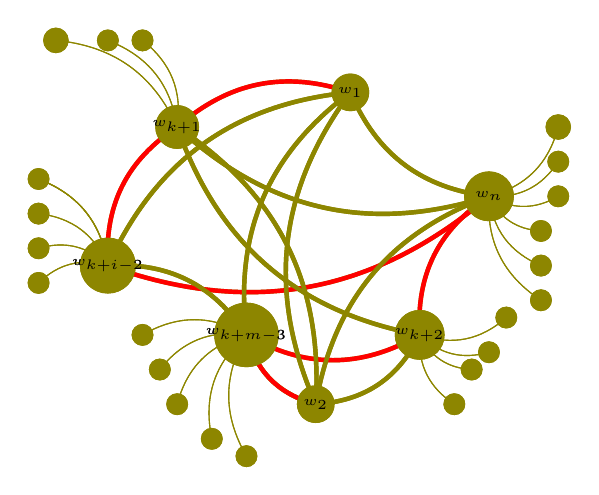
\begin{tikzpicture}[scale=0.22]

\draw[-,>=latex,ultra thick,color=olive] (14,2) to [bend left] (10,6);
\draw[-,>=latex,ultra thick,color=olive] (14,2) to [bend right] (20,6);
\draw[-,>=latex,ultra thick,color=olive] (10,6) to [bend right] (2,10);
\draw[-, >=latex,ultra thick,color=olive] (2,10) to [bend left] (6,18);
\draw[-, >=latex,ultra thick,>=latex,ultra thick,color=olive] (20,6) to [bend left] (24,14);
\draw[-,>=latex,ultra thick, >=latex,ultra thick,color=olive] (6,18) to [bend left] (16,20);
\draw[-,>=latex,ultra thick,color=olive] (16,20) to [bend right] (24,14);

\draw[-,>=latex,ultra thick,color=olive] (16,20) to [bend right] (2,10);
\draw[-,>=latex,ultra thick,color=olive] (16,20) to [bend right] (10,6);
\draw[-,>=latex,ultra thick,color=olive] (6,18) to [bend left] (14,2);
\draw[-, >=latex,ultra thick,color=olive] (2,10) to [bend right] (24,14);
\draw[-, >=latex,ultra thick,color=olive] (10,6) to [bend right] (20,6);
\draw[-,>=latex,ultra thick,color=olive] (24,14) to [bend right] (14,2);
\draw[-,>=latex,ultra thick,color=olive] (16,20) to [bend right] (14,2);
\draw[-,>=latex,ultra thick,color=olive] (6,18) to [bend right] (20,6);
\draw[-,>=latex,ultra thick,color=olive] (6,18) to [bend right] (24,14);
\draw[-, >=latex,ultra thick,color=olive] (10,6) to [bend right] (14,2);





\draw[-,color=olive] (6,18) to [bend right](-1,23);
\draw[-,color=olive] (6,18) to [bend right] (2,23);
\draw[-,color=olive] (6,18) to [bend right] (4,23);




\draw[-,color=olive] (20,6) to [bend right](22,2);
\draw[-,color=olive] (20,6) to [bend right] (23,4);
\draw[-,color=olive] (20,6) to [bend right] (24,5);
\draw[-,color=olive] (20,6) to [bend right] (25,7);


\draw[-,color=olive] (2,10) to [bend right](-2,9);
\draw[-,color=olive] (2,10) to [bend right] (-2,11);
\draw[-,color=olive] (2,10) to [bend right] (-2,13);
\draw[-,color=olive] (2,10) to [bend right] (-2,15);
\draw[-,color=olive] (2,10) to [bend right] (-2,15);




\draw[-,color=olive] (10,6) to [bend right](10,-1);
\draw[-,color=olive] (10,6) to [bend right] (8,0);
\draw[-,color=olive] (10,6) to [bend right] (6,2);
\draw[-,color=olive] (10,6) to [bend right] (5,4);
\draw[-,color=olive] (10,6) to [bend right] (4,6);




\draw[-,color=olive] (24,14) to [bend right](27,8);
\draw[-,color=olive] (24,14) to [bend right] (27,10);
\draw[-,color=olive] (24,14) to [bend right] (27,12);
\draw[-,color=olive] (24,14) to [bend right] (28,14);
\draw[-,color=olive] (24,14) to [bend right] (28,16);
\draw[-,color=olive] (24,14) to [bend right] (28,18);



\filldraw[color=olive] (-1,23) circle (20pt);% node[] {\small \textcolor{black}{$w_3$}};
\filldraw[color=olive] (2,23) circle (17pt);% node[] %{\tiny \textcolor{black}{$w_4$}};
\filldraw[color=olive] (4,23) circle (17pt);% node[] %{\tiny \textcolor{black}{$w_2$}};


\filldraw[color=olive] (-2,9) circle (17pt);% node[] {\tiny \textcolor{black}{$w$}};
\filldraw[color=olive] (-2,11) circle (17pt);% node[] %{\tiny \textcolor{black}{$w_4$}};
\filldraw[color=olive] (-2,13) circle (17pt);% node[] %{\tiny \textcolor{black}{$w_2$}};
\filldraw[color=olive] (-2,15) circle (17pt);% node[] %{\tiny \textcolor{black}{$w_2$}};

\filldraw[color=olive] (10,-1) circle (17pt);% node[] {\tiny \textcolor{black}{$w$}};
\filldraw[color=olive] (8,0) circle (17pt);% node[] %{\tiny \textcolor{black}{$w_4$}};
\filldraw[color=olive] (6,2) circle (17pt);% node[] %{\tiny \textcolor{black}{$w_2$}};
\filldraw[color=olive] (5,4) circle (17pt);% node[] %{\tiny \textcolor{black}{$w_2$}};
\filldraw[color=olive] (4,6) circle (17pt);% node[] %{\tiny \textcolor{black}{$w_2$}};



\filldraw[color=olive] (22,2) circle (17pt);% node[] {\tiny \textcolor{black}{$w$}};
\filldraw[color=olive] (23,4) circle (17pt);% node[] %{\tiny \textcolor{black}{$w_4$}};
\filldraw[color=olive] (24,5) circle (17pt);% node[] %{\tiny \textcolor{black}{$w_2$}};
\filldraw[color=olive] (25,7) circle (17pt);% node[] %{\tiny \textcolor{black}{$w_2$}};





\filldraw[color=olive] (27,8) circle (17pt);% node[] {\tiny \textcolor{black}{$w$}};
\filldraw[color=olive] (27,10) circle (17pt);% node[] %{\tiny \textcolor{black}{$w_4$}};
\filldraw[color=olive] (27,12) circle (17pt);% node[] %{\tiny \textcolor{black}{$w_2$}};
\filldraw[color=olive] (28,14) circle (17pt);% node[] %{\tiny \textcolor{black}{$w_2$}};
\filldraw[color=olive] (28,16) circle (17pt);% node[] %{\tiny \textcolor{black}{$w_2$}};



\filldraw[color=olive] (16,20) circle (30pt) node[] {\tiny \textcolor{black}{$w_1$}};
\filldraw[color=olive] (14,2) circle (30pt) node[] {\tiny\textcolor{black}{$w_2$}};
\filldraw[color=olive] (28,18) circle (20pt);% node[] {\small \textcolor{black}{$w_k$}};
\filldraw[color=olive] (6,18) circle (35pt) node[] {\tiny \textcolor{black}{$w_{k+1}$}};
\filldraw[color=olive] (20,6) circle (40pt) node[] {\tiny\textcolor{black}{$w_{k+2}$}};
\filldraw[color=olive] (2,10) circle (45pt) node[] {\tiny\textcolor{black}{$w_{k+i-2}$}};
\filldraw[color=olive] (10,6) circle (52pt) node[] {\tiny\textcolor{black}{$w_{k+m-3}$}};
%\filldraw[color=olive] (24,14) circle (40pt) node[] {\tiny \textcolor{black}{$w_{k+m-2}$}};
\filldraw[color=olive] (24,14) circle (40pt) node[] {\tiny\textcolor{black}{$w_{n}$}};


\pause
\draw[-, >=latex,ultra thick,color=red] (2,10) to [bend left] (6,18);
\draw[-, >=latex,ultra thick,color=red] (20,6) to [bend left] (24,14);
\draw[-, >=latex,ultra thick,color=red] (6,18) to [bend left] (16,20);
\draw[-, >=latex,ultra thick,color=red] (2,10) to [bend right] (24,14);
\draw[-, >=latex,ultra thick,color=red] (10,6) to [bend right] (20,6);
\draw[-, >=latex,ultra thick,color=red] (10,6) to [bend right] (14,2);



%\draw[-,>=latex,ultra thick,color=olive] (14,2) to [bend left] (10,6);
\draw[-,>=latex,ultra thick,color=olive] (14,2) to [bend right] (20,6);
\draw[-,>=latex,ultra thick,color=olive] (10,6) to [bend right] (2,10);
%\draw[-, >=latex,ultra thick,color=olive] (2,10) to [bend left] (6,18);
%\draw[-, >=latex,ultra thick,>=latex,ultra thick,color=olive] (20,6) to [bend left] (24,14);
%\draw[-,>=latex,ultra thick, >=latex,ultra thick,color=olive] (6,18) to [bend left] (16,20);
\draw[-,>=latex,ultra thick,color=olive] (16,20) to [bend right] (24,14);

\draw[-,>=latex,ultra thick,color=olive] (16,20) to [bend right] (2,10);
\draw[-,>=latex,ultra thick,color=olive] (16,20) to [bend right] (10,6);
\draw[-,>=latex,ultra thick,color=olive] (6,18) to [bend left] (14,2);
%\draw[-, >=latex,ultra thick,color=olive] (2,10) to [bend right] (24,14);
%\draw[-, >=latex,ultra thick,color=olive] (10,6) to [bend right] (20,6);
\draw[-,>=latex,ultra thick,color=olive] (24,14) to [bend right] (14,2);
\draw[-,>=latex,ultra thick,color=olive] (16,20) to [bend right] (14,2);
\draw[-,>=latex,ultra thick,color=olive] (6,18) to [bend right] (20,6);
\draw[-,>=latex,ultra thick,color=olive] (6,18) to [bend right] (24,14);
%\draw[-, >=latex,ultra thick,color=olive] (10,6) to [bend right] (14,2);





\draw[-,color=olive] (6,18) to [bend right](-1,23);
\draw[-,color=olive] (6,18) to [bend right] (2,23);
\draw[-,color=olive] (6,18) to [bend right] (4,23);




\draw[-,color=olive] (20,6) to [bend right](22,2);
\draw[-,color=olive] (20,6) to [bend right] (23,4);
\draw[-,color=olive] (20,6) to [bend right] (24,5);
\draw[-,color=olive] (20,6) to [bend right] (25,7);


\draw[-,color=olive] (2,10) to [bend right](-2,9);
\draw[-,color=olive] (2,10) to [bend right] (-2,11);
\draw[-,color=olive] (2,10) to [bend right] (-2,13);
\draw[-,color=olive] (2,10) to [bend right] (-2,15);
\draw[-,color=olive] (2,10) to [bend right] (-2,15);




\draw[-,color=olive] (10,6) to [bend right](10,-1);
\draw[-,color=olive] (10,6) to [bend right] (8,0);
\draw[-,color=olive] (10,6) to [bend right] (6,2);
\draw[-,color=olive] (10,6) to [bend right] (5,4);
\draw[-,color=olive] (10,6) to [bend right] (4,6);




\draw[-,color=olive] (24,14) to [bend right](27,8);
\draw[-,color=olive] (24,14) to [bend right] (27,10);
\draw[-,color=olive] (24,14) to [bend right] (27,12);
\draw[-,color=olive] (24,14) to [bend right] (28,14);
\draw[-,color=olive] (24,14) to [bend right] (28,16);
\draw[-,color=olive] (24,14) to [bend right] (28,18);



\filldraw[color=olive] (-1,23) circle (20pt);% node[] {\small \textcolor{black}{$w_3$}};
\filldraw[color=olive] (2,23) circle (17pt);% node[] %{\tiny \textcolor{black}{$w_4$}};
\filldraw[color=olive] (4,23) circle (17pt);% node[] %{\tiny \textcolor{black}{$w_2$}};


\filldraw[color=olive] (-2,9) circle (17pt);% node[] {\tiny \textcolor{black}{$w$}};
\filldraw[color=olive] (-2,11) circle (17pt);% node[] %{\tiny \textcolor{black}{$w_4$}};
\filldraw[color=olive] (-2,13) circle (17pt);% node[] %{\tiny \textcolor{black}{$w_2$}};
\filldraw[color=olive] (-2,15) circle (17pt);% node[] %{\tiny \textcolor{black}{$w_2$}};

\filldraw[color=olive] (10,-1) circle (17pt);% node[] {\tiny \textcolor{black}{$w$}};
\filldraw[color=olive] (8,0) circle (17pt);% node[] %{\tiny \textcolor{black}{$w_4$}};
\filldraw[color=olive] (6,2) circle (17pt);% node[] %{\tiny \textcolor{black}{$w_2$}};
\filldraw[color=olive] (5,4) circle (17pt);% node[] %{\tiny \textcolor{black}{$w_2$}};
\filldraw[color=olive] (4,6) circle (17pt);% node[] %{\tiny \textcolor{black}{$w_2$}};



\filldraw[color=olive] (22,2) circle (17pt);% node[] {\tiny \textcolor{black}{$w$}};
\filldraw[color=olive] (23,4) circle (17pt);% node[] %{\tiny \textcolor{black}{$w_4$}};
\filldraw[color=olive] (24,5) circle (17pt);% node[] %{\tiny \textcolor{black}{$w_2$}};
\filldraw[color=olive] (25,7) circle (17pt);% node[] %{\tiny \textcolor{black}{$w_2$}};





\filldraw[color=olive] (27,8) circle (17pt);% node[] {\tiny \textcolor{black}{$w$}};
\filldraw[color=olive] (27,10) circle (17pt);% node[] %{\tiny \textcolor{black}{$w_4$}};
\filldraw[color=olive] (27,12) circle (17pt);% node[] %{\tiny \textcolor{black}{$w_2$}};
\filldraw[color=olive] (28,14) circle (17pt);% node[] %{\tiny \textcolor{black}{$w_2$}};
\filldraw[color=olive] (28,16) circle (17pt);% node[] %{\tiny \textcolor{black}{$w_2$}};



\filldraw[color=olive] (16,20) circle (30pt) node[] {\tiny \textcolor{black}{$w_1$}};
\filldraw[color=olive] (14,2) circle (30pt) node[] {\tiny\textcolor{black}{$w_2$}};
\filldraw[color=olive] (28,18) circle (20pt);% node[] {\small \textcolor{black}{$w_k$}};
\filldraw[color=olive] (6,18) circle (35pt) node[] {\tiny \textcolor{black}{$w_{k+1}$}};
\filldraw[color=olive] (20,6) circle (40pt) node[] {\tiny\textcolor{black}{$w_{k+2}$}};
\filldraw[color=olive] (2,10) circle (45pt) node[] {\tiny\textcolor{black}{$w_{k+i-2}$}};
\filldraw[color=olive] (10,6) circle (52pt) node[] {\tiny\textcolor{black}{$w_{k+m-3}$}};
%\filldraw[color=olive] (24,14) circle (40pt) node[] {\tiny \textcolor{black}{$w_{k+m-2}$}};
\filldraw[color=olive] (24,14) circle (40pt) node[] {\tiny\textcolor{black}{$w_{n}$}};



\end{tikzpicture}
\end{center}
\end{figure}
\end{frame}
%%%%%%%%%%%%%%%%%%%%%%%%%%%%%%%%%%%%%%%%%%%%%%%%%%%%%%%%%%%%%%%%%%%
%%%%%%%%%%%%%%%%%%%%%%%%%%%%%%%%%%%%%%%%%%%%%%%%%%%%%%%%%%%%%%%%%%%%%
\begin{frame}
\frametitle{Demostraci�n}

\small {$T= H_{w_1 w_2} \cup (E(G) \text {\textbackslash} E(F))$ subgr�fica de $G_n$ es el �rbol generador deseado de $G_n$}
\begin{figure}[!ht]
\begin{center}
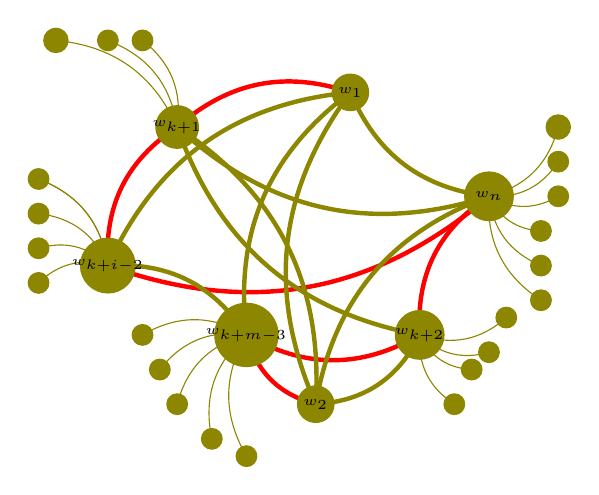
\begin{tikzpicture}[scale=0.22]



\pause
\draw[-, >=latex,ultra thick,color=red] (2,10) to [bend left] (6,18);
\draw[-, >=latex,ultra thick,color=red] (20,6) to [bend left] (24,14);
\draw[-, >=latex,ultra thick,color=red] (6,18) to [bend left] (16,20);
\draw[-, >=latex,ultra thick,color=red] (2,10) to [bend right] (24,14);
\draw[-, >=latex,ultra thick,color=red] (10,6) to [bend right] (20,6);
\draw[-, >=latex,ultra thick,color=red] (10,6) to [bend right] (14,2);



%\draw[-,>=latex,ultra thick,color=olive] (14,2) to [bend left] (10,6);
\draw[-,>=latex,ultra thick,color=olive] (14,2) to [bend right] (20,6);
\draw[-,>=latex,ultra thick,color=olive] (10,6) to [bend right] (2,10);
%\draw[-, >=latex,ultra thick,color=olive] (2,10) to [bend left] (6,18);
%\draw[-, >=latex,ultra thick,>=latex,ultra thick,color=olive] (20,6) to [bend left] (24,14);
%\draw[-,>=latex,ultra thick, >=latex,ultra thick,color=olive] (6,18) to [bend left] (16,20);
\draw[-,>=latex,ultra thick,color=olive] (16,20) to [bend right] (24,14);

\draw[-,>=latex,ultra thick,color=olive] (16,20) to [bend right] (2,10);
\draw[-,>=latex,ultra thick,color=olive] (16,20) to [bend right] (10,6);
\draw[-,>=latex,ultra thick,color=olive] (6,18) to [bend left] (14,2);
%\draw[-, >=latex,ultra thick,color=olive] (2,10) to [bend right] (24,14);
%\draw[-, >=latex,ultra thick,color=olive] (10,6) to [bend right] (20,6);
\draw[-,>=latex,ultra thick,color=olive] (24,14) to [bend right] (14,2);
\draw[-,>=latex,ultra thick,color=olive] (16,20) to [bend right] (14,2);
\draw[-,>=latex,ultra thick,color=olive] (6,18) to [bend right] (20,6);
\draw[-,>=latex,ultra thick,color=olive] (6,18) to [bend right] (24,14);
%\draw[-, >=latex,ultra thick,color=olive] (10,6) to [bend right] (14,2);





\draw[-,color=olive] (6,18) to [bend right](-1,23);
\draw[-,color=olive] (6,18) to [bend right] (2,23);
\draw[-,color=olive] (6,18) to [bend right] (4,23);




\draw[-,color=olive] (20,6) to [bend right](22,2);
\draw[-,color=olive] (20,6) to [bend right] (23,4);
\draw[-,color=olive] (20,6) to [bend right] (24,5);
\draw[-,color=olive] (20,6) to [bend right] (25,7);


\draw[-,color=olive] (2,10) to [bend right](-2,9);
\draw[-,color=olive] (2,10) to [bend right] (-2,11);
\draw[-,color=olive] (2,10) to [bend right] (-2,13);
\draw[-,color=olive] (2,10) to [bend right] (-2,15);
\draw[-,color=olive] (2,10) to [bend right] (-2,15);




\draw[-,color=olive] (10,6) to [bend right](10,-1);
\draw[-,color=olive] (10,6) to [bend right] (8,0);
\draw[-,color=olive] (10,6) to [bend right] (6,2);
\draw[-,color=olive] (10,6) to [bend right] (5,4);
\draw[-,color=olive] (10,6) to [bend right] (4,6);




\draw[-,color=olive] (24,14) to [bend right](27,8);
\draw[-,color=olive] (24,14) to [bend right] (27,10);
\draw[-,color=olive] (24,14) to [bend right] (27,12);
\draw[-,color=olive] (24,14) to [bend right] (28,14);
\draw[-,color=olive] (24,14) to [bend right] (28,16);
\draw[-,color=olive] (24,14) to [bend right] (28,18);



\filldraw[color=olive] (-1,23) circle (20pt);% node[] {\small \textcolor{black}{$w_3$}};
\filldraw[color=olive] (2,23) circle (17pt);% node[] %{\tiny \textcolor{black}{$w_4$}};
\filldraw[color=olive] (4,23) circle (17pt);% node[] %{\tiny \textcolor{black}{$w_2$}};


\filldraw[color=olive] (-2,9) circle (17pt);% node[] {\tiny \textcolor{black}{$w$}};
\filldraw[color=olive] (-2,11) circle (17pt);% node[] %{\tiny \textcolor{black}{$w_4$}};
\filldraw[color=olive] (-2,13) circle (17pt);% node[] %{\tiny \textcolor{black}{$w_2$}};
\filldraw[color=olive] (-2,15) circle (17pt);% node[] %{\tiny \textcolor{black}{$w_2$}};

\filldraw[color=olive] (10,-1) circle (17pt);% node[] {\tiny \textcolor{black}{$w$}};
\filldraw[color=olive] (8,0) circle (17pt);% node[] %{\tiny \textcolor{black}{$w_4$}};
\filldraw[color=olive] (6,2) circle (17pt);% node[] %{\tiny \textcolor{black}{$w_2$}};
\filldraw[color=olive] (5,4) circle (17pt);% node[] %{\tiny \textcolor{black}{$w_2$}};
\filldraw[color=olive] (4,6) circle (17pt);% node[] %{\tiny \textcolor{black}{$w_2$}};



\filldraw[color=olive] (22,2) circle (17pt);% node[] {\tiny \textcolor{black}{$w$}};
\filldraw[color=olive] (23,4) circle (17pt);% node[] %{\tiny \textcolor{black}{$w_4$}};
\filldraw[color=olive] (24,5) circle (17pt);% node[] %{\tiny \textcolor{black}{$w_2$}};
\filldraw[color=olive] (25,7) circle (17pt);% node[] %{\tiny \textcolor{black}{$w_2$}};





\filldraw[color=olive] (27,8) circle (17pt);% node[] {\tiny \textcolor{black}{$w$}};
\filldraw[color=olive] (27,10) circle (17pt);% node[] %{\tiny \textcolor{black}{$w_4$}};
\filldraw[color=olive] (27,12) circle (17pt);% node[] %{\tiny \textcolor{black}{$w_2$}};
\filldraw[color=olive] (28,14) circle (17pt);% node[] %{\tiny \textcolor{black}{$w_2$}};
\filldraw[color=olive] (28,16) circle (17pt);% node[] %{\tiny \textcolor{black}{$w_2$}};



\filldraw[color=olive] (16,20) circle (30pt) node[] {\tiny \textcolor{black}{$w_1$}};
\filldraw[color=olive] (14,2) circle (30pt) node[] {\tiny\textcolor{black}{$w_2$}};
\filldraw[color=olive] (28,18) circle (20pt);% node[] {\small \textcolor{black}{$w_k$}};
\filldraw[color=olive] (6,18) circle (35pt) node[] {\tiny \textcolor{black}{$w_{k+1}$}};
\filldraw[color=olive] (20,6) circle (40pt) node[] {\tiny\textcolor{black}{$w_{k+2}$}};
\filldraw[color=olive] (2,10) circle (45pt) node[] {\tiny\textcolor{black}{$w_{k+i-2}$}};
\filldraw[color=olive] (10,6) circle (52pt) node[] {\tiny\textcolor{black}{$w_{k+m-3}$}};
%\filldraw[color=olive] (24,14) circle (40pt) node[] {\tiny \textcolor{black}{$w_{k+m-2}$}};
\filldraw[color=olive] (24,14) circle (40pt) node[] {\tiny\textcolor{black}{$w_{n}$}};



\end{tikzpicture}
\end{center}
\end{figure}
\end{frame}


%%%%%%%%%%%%%%%%%%%%%%%%%%%%%%%%%%%%%%%%%%%%%%%%%%%%%555
%%%%%%%%%%%%%%%%%%%%%%%%%%%%%%%%%%%%%%%%%%%%%%%%%%%%%%%555
\begin{frame}
\frametitle{Demostraci�n}

\small {\textcolor{blue}{$T= H_{w_1 w_2} \cup (E(G) \text {\textbackslash} E(F))$} subgr�fica de \textcolor{blue}{$G_n$} es el �rbol generador deseado de \textcolor{blue}{$G_n$}}
\begin{figure}[!ht]
\begin{center}
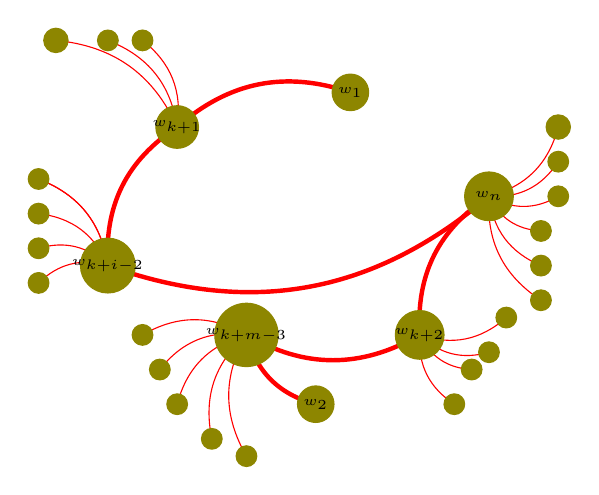
\begin{tikzpicture}[scale=0.22]


\draw[-, >=latex,ultra thick,color=red] (2,10) to [bend left] (6,18);
\draw[-, >=latex,ultra thick,color=red] (20,6) to [bend left] (24,14);
\draw[-, >=latex,ultra thick,color=red] (6,18) to [bend left] (16,20);
\draw[-, >=latex,ultra thick,color=red] (2,10) to [bend right] (24,14);
\draw[-, >=latex,ultra thick,color=red] (10,6) to [bend right] (20,6);
\draw[-, >=latex,ultra thick,color=red] (10,6) to [bend right] (14,2);




%\draw[-,>=latex,ultra thick,color=olive] (14,2) to [bend right] (20,6);
%\draw[-,>=latex,ultra thick,color=olive] (10,6) to [bend right] (2,10);
%
%\draw[-,>=latex,ultra thick,color=olive] (16,20) to [bend right] (24,14);
%
%\draw[-,>=latex,ultra thick,color=olive] (16,20) to [bend right] (2,10);
%\draw[-,>=latex,ultra thick,color=olive] (16,20) to [bend right] (10,6);
%\draw[-,>=latex,ultra thick,color=olive] (6,18) to [bend left] (14,2);
%
%\draw[-,>=latex,ultra thick,color=olive] (24,14) to [bend right] (14,2);
%\draw[-,>=latex,ultra thick,color=olive] (16,20) to [bend right] (14,2);
%\draw[-,>=latex,ultra thick,color=olive] (6,18) to [bend right] (20,6);
%\draw[-,>=latex,ultra thick,color=olive] (6,18) to [bend right] (24,14);






\draw[-,color=red] (6,18) to [bend right](-1,23);
\draw[-,color=red] (6,18) to [bend right] (2,23);
\draw[-,color=red] (6,18) to [bend right] (4,23);




\draw[-,color=red] (20,6) to [bend right](22,2);
\draw[-,color=red] (20,6) to [bend right] (23,4);
\draw[-,color=red] (20,6) to [bend right] (24,5);
\draw[-,color=red] (20,6) to [bend right] (25,7);


\draw[-,color=red] (2,10) to [bend right](-2,9);
\draw[-,color=red] (2,10) to [bend right] (-2,11);
\draw[-,color=red] (2,10) to [bend right] (-2,13);
\draw[-,color=red] (2,10) to [bend right] (-2,15);
\draw[-,color=red] (2,10) to [bend right] (-2,15);




\draw[-,color=red] (10,6) to [bend right](10,-1);
\draw[-,color=red] (10,6) to [bend right] (8,0);
\draw[-,color=red] (10,6) to [bend right] (6,2);
\draw[-,color=red] (10,6) to [bend right] (5,4);
\draw[-,color=red] (10,6) to [bend right] (4,6);




\draw[-,color=red] (24,14) to [bend right](27,8);
\draw[-,color=red] (24,14) to [bend right] (27,10);
\draw[-,color=red] (24,14) to [bend right] (27,12);
\draw[-,color=red] (24,14) to [bend right] (28,14);
\draw[-,color=red] (24,14) to [bend right] (28,16);
\draw[-,color=red] (24,14) to [bend right] (28,18);



\filldraw[color=olive] (-1,23) circle (20pt);% node[] {\small \textcolor{black}{$w_3$}};
\filldraw[color=olive] (2,23) circle (17pt);% node[] %{\tiny \textcolor{black}{$w_4$}};
\filldraw[color=olive] (4,23) circle (17pt);% node[] %{\tiny \textcolor{black}{$w_2$}};


\filldraw[color=olive] (-2,9) circle (17pt);% node[] {\tiny \textcolor{black}{$w$}};
\filldraw[color=olive] (-2,11) circle (17pt);% node[] %{\tiny \textcolor{black}{$w_4$}};
\filldraw[color=olive] (-2,13) circle (17pt);% node[] %{\tiny \textcolor{black}{$w_2$}};
\filldraw[color=olive] (-2,15) circle (17pt);% node[] %{\tiny \textcolor{black}{$w_2$}};

\filldraw[color=olive] (10,-1) circle (17pt);% node[] {\tiny \textcolor{black}{$w$}};
\filldraw[color=olive] (8,0) circle (17pt);% node[] %{\tiny \textcolor{black}{$w_4$}};
\filldraw[color=olive] (6,2) circle (17pt);% node[] %{\tiny \textcolor{black}{$w_2$}};
\filldraw[color=olive] (5,4) circle (17pt);% node[] %{\tiny \textcolor{black}{$w_2$}};
\filldraw[color=olive] (4,6) circle (17pt);% node[] %{\tiny \textcolor{black}{$w_2$}};



\filldraw[color=olive] (22,2) circle (17pt);% node[] {\tiny \textcolor{black}{$w$}};
\filldraw[color=olive] (23,4) circle (17pt);% node[] %{\tiny \textcolor{black}{$w_4$}};
\filldraw[color=olive] (24,5) circle (17pt);% node[] %{\tiny \textcolor{black}{$w_2$}};
\filldraw[color=olive] (25,7) circle (17pt);% node[] %{\tiny \textcolor{black}{$w_2$}};





\filldraw[color=olive] (27,8) circle (17pt);% node[] {\tiny \textcolor{black}{$w$}};
\filldraw[color=olive] (27,10) circle (17pt);% node[] %{\tiny \textcolor{black}{$w_4$}};
\filldraw[color=olive] (27,12) circle (17pt);% node[] %{\tiny \textcolor{black}{$w_2$}};
\filldraw[color=olive] (28,14) circle (17pt);% node[] %{\tiny \textcolor{black}{$w_2$}};
\filldraw[color=olive] (28,16) circle (17pt);% node[] %{\tiny \textcolor{black}{$w_2$}};



\filldraw[color=olive] (16,20) circle (30pt) node[] {\tiny \textcolor{black}{$w_1$}};
\filldraw[color=olive] (14,2) circle (30pt) node[] {\tiny\textcolor{black}{$w_2$}};
\filldraw[color=olive] (28,18) circle (20pt);% node[] {\small \textcolor{black}{$w_k$}};
\filldraw[color=olive] (6,18) circle (35pt) node[] {\tiny \textcolor{black}{$w_{k+1}$}};
\filldraw[color=olive] (20,6) circle (40pt) node[] {\tiny\textcolor{black}{$w_{k+2}$}};
\filldraw[color=olive] (2,10) circle (45pt) node[] {\tiny\textcolor{black}{$w_{k+i-2}$}};
\filldraw[color=olive] (10,6) circle (52pt) node[] {\tiny\textcolor{black}{$w_{k+m-3}$}};
%\filldraw[color=olive] (24,14) circle (40pt) node[] {\tiny \textcolor{black}{$w_{k+m-2}$}};
\filldraw[color=olive] (24,14) circle (40pt) node[] {\tiny\textcolor{black}{$w_{n}$}};

\end{tikzpicture}
\end{center}
\end{figure}
\end{frame}


\begin{frame}

Si la gr�fica \textcolor{blue}{$G$} con \textcolor{blue} {$V(G)=\{ w_1, w_2,w_3, \ldots, w_n \}$} tiene un �rbol generador \textcolor{blue} {$T$} tal que \textcolor{blue}{$d_T (w_i)= d_i$} con \textcolor{blue}{$1 \leq i \leq n$}, entonces la gr�fica \textcolor{blue}{$G^*$} tiene una trayectoria hamiltoniana con v�rtice inicial \textcolor{blue}{$v_1$} y v�rtice final \textcolor{blue}{$v_2$}.

\end{frame}

\begin{frame}
Finalmente, veamos que al hacer $G_n=f(G_m)$, $k-2=|G_n|$\textbackslash $|G_m|$ es el n�mero de v�rtices que se le pega a $G_m$ y dado que cada uno de estos v�rtices nuevos es adyacente a un $v_i$ de $G_m$ con $3\leq i \leq m$ se usan $k-2=|E(G_n)|$\textbackslash $|E(G_m)|$ aristas para hacer esto y el n�mero de v�rtices que se reetiquetan son $m$. Por lo cual el trabajo que realiza la tranformaci�n $f$ es $2(k-2)+m \leq 2n$ en un tiempo lineal. 
 
\end{frame}
